\documentclass{article}
%% Useful packages
\usepackage[utf8]{inputenc}
\usepackage[a4paper,left=2cm,right=2cm,top=2cm,bottom=2cm]{geometry}
\usepackage{crop,graphicx,amsmath,array,color,amssymb,fancyhdr,lineno,bm}
\usepackage{flushend,stfloats,amsthm,chngpage,times,,lipsum,lastpage} 
\usepackage{calc,listings,color,wrapfig,tabularx,longtable,enumitem}
\usepackage[style=numeric-comp,backend=biber]{biblatex}
\addbibresource{Refs.bib}
\usepackage{lineno}
%%%%%%%%%%%%   Header and Footer  %%%%%%%%%%%%%
\pagestyle{fancy}
\fancypagestyle{plain}{%
  \renewcommand{\headrulewidth}{0pt}%
  \fancyhf{}%
}

\title{%
  First Assignment \\
  \large Equivalent representations of orientation matrices}
\author{Surname Name}

\begin{document}
\begin{titlepage}

\newcommand{\HRule}{\rule{\linewidth}{0.5mm}} % Defines a new command for the horizontal lines, change thickness here

%----------------------------------------------------------------------------------------
%	LOGO SECTION
%----------------------------------------------------------------------------------------
\center

\includegraphics[width=5cm]{Title/Unige-logo.jpeg}\\[1cm] % Include a department/university logo - this will require the graphicx package
 
%----------------------------------------------------------------------------------------

\center % Center everything on the page

%----------------------------------------------------------------------------------------
%	HEADING SECTIONS
%----------------------------------------------------------------------------------------

\textsc{\Huge Università degli studi di Genova}\\[1cm] % Name of your university/college
\textsc{\LARGE DIBRIS}\\[0.3cm]
\textsc{\Small Department of Computer Science and Technology,}\\
\textsc{\Small Bioengineering, Robotics and System Engineering}\\[1cm] % Minor heading such as course title
\textsc{\LARGE{Modelling and Control of Manipulators}}\\[1cm] % Major heading such as course name

%----------------------------------------------------------------------------------------
%	TITLE SECTION
%----------------------------------------------------------------------------------------
\makeatletter
\HRule \\[0.4cm]
{ \huge \bfseries First Assignment}\\[0.2cm] 
{\Large \bfseries Equivalent representations of orientation matrices}\\
% Title of your document
\HRule \\[1.5cm]
 
%----------------------------------------------------------------------------------------
%	AUTHOR SECTION
%----------------------------------------------------------------------------------------

\begin{minipage}{0.4\textwidth}
\begin{flushleft} \large
\emph{Author:}\\[0.2cm]
Surname Name % Your name
\\[1.2em]
\emph{Student ID:}\\[0.2cm]
s0000000 \\[1.2em]
\end{flushleft}
\end{minipage}
~
\begin{minipage}{0.4\textwidth}
\begin{flushright} \large
\emph{Professors:} \\[0.2cm]
Enrico Simetti\\
Giorgio Cannata  \\[1.2em] % Supervisor's Name

\emph{Tutors:} \\[0.2cm]
Andrea Tiranti\\
Francesco Giovinazzo\\
George Kurshakov
% second marker's name
\end{flushright}
\end{minipage}\\[2cm]
\makeatother

% If you don't want a supervisor, uncomment the two lines below and remove the section above
%\Large \emph{Author:}\\
%John \textsc{Smith}\\[3cm] % Your name

%----------------------------------------------------------------------------------------
%	DATE SECTION
%----------------------------------------------------------------------------------------

{\large \today}\\[2cm] % Date, change the \today to a set date if you want to be precise

\vfill % Fill the rest of the page with whitespace

\end{titlepage}

\sffamily

\fancyhf{}
\fancyhead[L]{Surname Name - s0000000}
\fancyhead[R]{Modelling and Control of Manipulators - Assignment 1}
\fancyfoot[R]{ \bf\thepage\ \rm }%

\newpage
\tableofcontents

\section*{}
\begin{longtable}{|p{4cm}|p{4cm}|p{4cm}|}
    \hline
    Mathematical expression & Definition & MATLAB expression \\
    \hline 
    $<w>$ & World Coordinate Frame &  w\\[0.4cm]
    $^a_b R$ & Rotation matrix of frame $<b>$ with respect to frame $<a>$  & aRb \\[1.2cm]
    $^a_b T$ & Transformation matrix of frame $<b>$ with respect to frame $<a>$ & aTb \\[1.2cm]
    \hline
    \caption{Nomenclature Table}
\end{longtable}

\section{Assignment description}
The first assignment of Modelling and Control of Manipulators focuses on the geometric fundamentals and algorithmic tools underlying any robotics application. The concepts of transformation matrix, orientation matrix and the equivalent representations of orientation matrices (Equivalent angle-axis representation, Euler Angles and Quaternions) will be reviewed.

The first assignment is \textbf{mandatory} and consists of 4 different exercises. You are asked to:
\begin{itemize}
    \item Download the .zip file called MOCOM-LAB1 from the Aulaweb page of this course.
    \item Implement the code to solve the exercises on MATLAB by filling the predefined files called "\textit{main.m}", "\textit{ComputeAngleAxis.m}", "\textit{ComputeInverseAngleAxis.m}", and "\textit{QuatToRot.m}".
    \item Write a report motivating the answers for each exercise, following the predefind format on this document.
\end{itemize}

\subsection{Exercise 1 - Equivalent Angle-Axis Representation (Exponential representation)}
A particularly interesting minimal representation of 3D rotation matrices is the so-called "\textit{angle-axis representation}" or "\textit{exponential representation}". Given two frames $<a>$ and $<b>$, initially coinciding, let's consider an applied geometric unit vector \begin{math}(\textbf{v},O_a) = (\textbf{v},O_b)\end{math}, passing through the common origin of the two frames, whose initial projection on $<a>$ is the same of that on $<b>$. Then let's consider that frame $<b>$ is purely rotated around $\textbf{v}$ of an angle $\theta$, even negative, accordingly with the right-hand rule. We note that the axis-line defined by \begin{math}(\textbf{v},O_a) = (\textbf{v},O_b)\end{math} remains common to both the reference systems of the two frames $<a>$ and $<b>$ and we obtain that the orientation matrix constructed in the above way is said to be represented by its equivalent angle-axis representation that admits the following equivalent analytical expression, also known as Rodrigues Formula:

\[ \textbf{R}(^* \textbf{v},\theta) = e^{[^*\textbf{v}\times]\theta} = e^{[\rho\times]} =  \textbf{I}_{3x3} + [^* \textbf{v}\times] \sin(\theta) + [^* \textbf{v}\times]^2 (1-\cos(\theta))\]

\textbf{Q1.1} Given two generic frames $<a>$ and $<b>$, given the geometric unit vector \begin{math}(\textbf{v},O_a) = (\textbf{v},O_b)\end{math} and the angle $\theta$, implement on MATLAB the Rodrigues formula, computing the rotation matrix $^a_b R$ of frame $<b>$  with respect to $<a>$ .

Then test it for the following cases and comment the results obtained, including some sketches of the frames configurations:
\begin{itemize}
    \item \textbf{Q1.2}\hspace{10mm} \begin{math} \textbf{v} = [1,0,0]\end{math} and  \begin{math} \theta = 45^\circ \end{math}
    \item \textbf{Q1.3}\hspace{10mm} \begin{math} \textbf{v} = [0,1,0]\end{math} and  \begin{math} \theta = \pi/6 \end{math}
    \item \textbf{Q1.4}\hspace{10mm} \begin{math} \textbf{v} = [0,0,1]\end{math} and  \begin{math} \theta = 3\pi/4 \end{math}
    \item \textbf{Q1.5}\hspace{10mm} \begin{math} \textbf{v}  = [0.3202,    0.5337,    0.7827]\end{math} and  \begin{math} \theta = 2.8 \end{math}
    \item \textbf{Q1.6}\hspace{10mm} \begin{math} \bm{\rho} = [0, 2\pi/3, 0];\end{math}
    \item \textbf{Q1.7}\hspace{10mm} \begin{math} \bm{\rho} = [0.25, -1.3, 0.15];\end{math}
    \item \textbf{Q1.8}\hspace{10mm} \begin{math} \bm{\rho} = [-\pi/4, -\pi/3 ,\pi/6];\end{math}
\end{itemize}
\textbf{Note that $\bm{\rho}$ is $\bm{\rho} = \textbf{v}*\theta$}
\subsection{Exercise 2 - Inverse Equivalent Angle-Axis Problem}
Given two reference frames $<a>$ and $<b>$, referred to a common world coordinate system $<w>$, their orientation with respect to the world frame $<w>$ is expressed in Figure \ref{fig:ex2}.
\newline

\begin{figure}
\centering
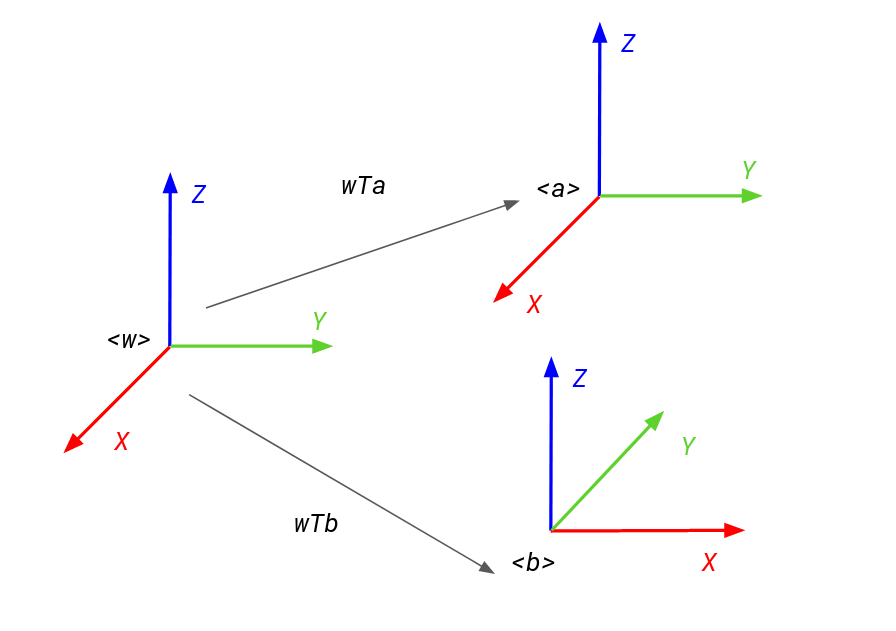
\includegraphics[width=0.6\linewidth]{Resources/reference_frames_ex2.png}
\caption{exercise 2 frames}
\label{fig:ex2}
\end{figure}

\textbf{Q2.1} Compute the orientation matrix $^a_b R$, by inspection of Figure 1, without using the Rodriguez formula. 

\textbf{Q2.2} Solve the Inverse Equivalent Angle-Axis Problem for the orientation matrix $^a_b R$.

\textbf{Q2.3} Given the following Transformation matrix:

 $^w_c T =\begin{bmatrix}
0.835959 & -0.283542 & -0.46986 & 0\\
    0.271321 & 0.957764 & -0.0952472 & -1.23\\
    0.47703 & -0.0478627 & 0.877583 & 14\\
    0 & 0 & 0 & 1
\end{bmatrix}$

Solve the Inverse Equivalent Angle-Axis Problem for the orientation matrix $^c_b R$.

\newpage
\subsection{Exercise 3 - Euler angles (Z-X-Z) vs Tait-Bryan angles (Yaw-Pitch-Roll)}
Any orientation matrix can be expressed in terms of three elementary rotations in sequence. These can occur either about the axes of a fixed coordinate system (extrinsic rotations), or about the axes of a rotating coordinate system (intrinsic rotations) initially aligned with the fixed one. Then we can distinguish:
\begin{itemize}
    \item Proper Euler angles: X-Z-X, Y-Z-Y, ...
    \item Tait-Bryan angles: Z-Y-X, X-Y-Z, ...
\end{itemize}

\textbf{Q3.1} Given two generic frames $<w>$ and $<b>$, define the elementary orientation matrices for frame $<b>$ with respect to frame $<w>$, knowing that:
\begin{itemize}
    \item $<b>$ is rotated of $45^\circ$ around the z-axis of $<w>$
    \item $<b>$ is rotated of $60^\circ$ around the y-axis of $<w>$
    \item $<b>$ is rotated of $-30^\circ$ around the x-axis of $<w>$
\end{itemize}

\textbf{Q3.2} Compute the equivalent angle-axis representation for each elementary rotation

\textbf{Q3.3} Compute the z-y-x (yaw,pitch,roll) representation and solve the Inverse Equivalent Angle-Axis Problem for the obtained orientation matrix

\textbf{Q3.4} Compute the z-x-z representation and solve the Inverse Equivalent Angle-Axis Problem for the obtained orientation matrix

\subsection{Exercise 4 - Quaternions}
Given the following quaternion: $q = 0.1647 + 0.31583i + 0.52639j + 0.77204k$ expressing how a reference frame $<b>$ is rotated with respect to $<a>$:

\textbf{Q4.1} Compute the equivalent rotation matrix, \textbf{WITHOUT} using built-in matlab functions.

\textbf{Q4.2} Solve the Inverse Equivalent Angle-Axis Problem for the obtained orientation matrix

\newpage
\section{Exercise 1} \label{P1}
% Write some intro
\subsection{Q1.1}
\subsection{Q1.2}
\subsection{Q1.3}
\subsection{Q1.4}
\subsection{Q1.5}
\subsection{Q1.6}
\subsection{Q1.7}
\subsection{Q1.8}

\textit{[Comment] For each exercise include an image of the initial frames configuration, with the applied geometric unit vector and an image of the final configuration} 

\textit{[Comment] For each exercise report the results obtained and provide an explanation of the result obtained (even though it might seem trivial) } 
\section{Exercise 2} \label{P2}

\textit{[Comment] Same structure of exercise 1 } 
\section{Exercise 3} \label{P3}

\textit{[Comment] Same structure of exercise 1 } 

\section{Exercise 4} \label{P4}

\textit{[Comment] Same structure of exercise 1 } 


\pagebreak

\section{Appendix}
\textit{[Comment] Add here additional material (if needed)} 
\subsection{Appendix A}

\subsection{Appendix B}


\end{document}
